\documentclass[11pt]{article}
\usepackage{amsmath}
\usepackage{amssymb}
\usepackage{amsthm}
\usepackage{bm}
\usepackage{hyperref}
\usepackage[authoryear]{natbib}  % or [authoryear] for name-year style
\usepackage{graphicx}

\usepackage{algorithm}
\usepackage{algorithmic}
\usepackage{xcolor}

\theoremstyle{definition}
\newtheorem{definition}{Definition}

\newcommand{\avi}[1]{\textcolor{teal}{[Avi: #1]}}


\title{Bayesian Time-Varying Spectral Estimation in the Wavelet Domain\\
with Tensor-Product Log-P-Splines}
\author{}
\date{}

\begin{document}

\maketitle

\begin{abstract}
We estimate the power spectral density (PSD) of non-stationary noise directly in
the Wilson--Daubechies--Meyer (WDM) wavelet domain. Each WDM coefficient is
modelled as a zero-mean Gaussian whose variance is the local evolutionary power,
and the log-PSD surface is represented by a tensor-product P-spline with an
anisotropic roughness prior. We sample the prior in a non-centered (whitened)
form that diagonalizes the smoothing precision, eliminating the hierarchical
funnel that otherwise stalls Hamiltonian Monte Carlo. In simulation studies on a
locally stationary process and on a LISA-like instrument-plus-confusion noise
budget with a seasonally modulated Galactic foreground, the method recovers the
time-varying surface from a single realization with near-nominal credible
intervals and no sampler divergences. Because the likelihood is Gaussian on the
coefficients, it retains phase and admits a signal mean, so a gravitational-wave
signal and the non-stationary noise PSD can be inferred jointly; we demonstrate
this with a galactic binary injected into the modulated LISA noise.
\end{abstract}

\section{Model Specification}

\begin{definition}[Moving periodogram ordinates]
The \emph{moving periodogram ordinates} $\mathrm{MI}_t$ (of order $m$) at time point 
$t = 1, \ldots, T$ of $X_{t-m+1}, \ldots, X_{t+m}$ are defined by
\begin{equation}
\mathrm{MI}_t = \frac{1}{2\pi(2m+1)}
\left|
\sum_{\nu = 0}^{2m}
X_{\,\nu + t - m}\,
\exp\!\left(-i \pi \nu \lambda_{\mathrm{mod}(t)}\right)
\right|^2,
\label{eq:MI}
\end{equation}
where $\lambda_j = \frac{2j}{2m+1}$ for $j = 1, 2, \ldots, m$ are the Fourier frequencies and 
$\mathrm{mod}(t) = 1 + ((t - 1) \bmod m)$.
\end{definition}

\begin{definition}[Dynamic Whittle likelihood]
The \emph{dynamic Whittle likelihood} based on the moving periodogram ordinates is defined by
\begin{equation}
L^{(1)}_{\mathrm{DW}}(f)
=
\prod_{t = 1}^{T}
\frac{1}{f(t/T, \lambda_{\mathrm{mod}(t)})}
\exp\!\left(
-\frac{\mathrm{MI}_t}{f(t/T, \lambda_{\mathrm{mod}(t)})}
\right).
\label{eq:dynamic_whittle}
\end{equation}
\end{definition}

\begin{definition}[Thinned dynamic Whittle likelihood]
The \emph{thinned dynamic Whittle likelihood} with thinning factor $i = 2, 3$ is given by
\begin{equation}
L^{(i)}_{\mathrm{DW}}(f)
=
\prod_{l = 1}^{B_i}
\prod_{j = 1}^{m}
\frac{1}{f(u_{j,l,i}, \lambda_j)}
\exp\!\left(
-\frac{\mathrm{MI}(u_{j,l,i}, \lambda_j)}{f(u_{j,l,i}, \lambda_j)}
\right),
\label{eq:thinned_dynamic_whittle}
\end{equation}
where
\[
B_i = \left\lfloor \frac{T - m}{i m} \right\rfloor,
\qquad
u_{j,l,i} = \frac{i(l - 1)m + j}{T}.
\]
\end{definition}
\subsection{Joint Estimation of GW Signal}
Let the data be composed of GW signal and a locally stationary noise time series 
\[d(t)=h(t;\theta) + X(t)\]
and define the moving Fourier transform of $X$
\[ \tilde{X}_t(\lambda_{\mathrm{mod}(t)})=\frac{1}{\sqrt{2\pi(2m+1)}}
\sum_{\nu = 0}^{2m}
X_{\,\nu + t - m}\,
\exp\!\left(-i \pi \nu \lambda_{\mathrm{mod}(t)}\right)
\]

Let $\tilde{h}(\lambda \mid \theta)$ be the frequency representation of the GW signal.
\begin{definition}[Dynamic Whittle likelihood]
The \emph{dynamic Whittle likelihood} based on the moving periodogram ordinates is defined by
\begin{equation}
L^{(1)}_{\mathrm{DW}}(f,\theta)
=
\prod_{t = 1}^{T}
\frac{1}{f(t/T, \lambda_{\mathrm{mod}(t)})}
\exp\!\left(
-\frac{\left(\tilde{X}_t(\lambda_{\mathrm{mod}(t)}) - \tilde{h}(\lambda_{\mathrm{mod}(t)} \mid \theta)\right)^2}{f(t/T, \lambda_{\mathrm{mod}(t)})}
\right).
%\label{eq:dynamic_whittle}
\end{equation}
\end{definition}

%%%%%%%%%%%%%%%%%%%%%%%%%%%%%%%%%%%%%%%%%%%%%%%%%%%%%%%%%%%%%%%%%
\subsection{2D Tensor Product P-splines}

We model the log power spectral density as a smooth bivariate function using tensor product P-splines \citep{eilers2003multivariate, wood2017generalized}:

\begin{equation}
\log S(t_i, f_j) = \sum_{k=1}^{K_t} \sum_{l=1}^{K_f} w_{kl} B_k^{(t)}(t_i) B_l^{(f)}(f_j)
\end{equation}

where:
\begin{itemize}
\item $S(t_i, f_j)$ is the power spectral density at time $t_i$ and frequency $f_j$
\item $B_k^{(t)}(\cdot)$ are B-spline basis functions for time (degree $d_t$)
\item $B_l^{(f)}(\cdot)$ are B-spline basis functions for frequency (degree $d_f$)
\item $w_{kl}$ are the spline coefficients
\item $K_t = n_{\text{knots},t} + d_t - 1$ is the number of time basis functions
\item $K_f = n_{\text{knots},f} + d_f - 1$ is the number of frequency basis functions
\end{itemize}

In matrix notation:
\begin{equation}
\bm{\Lambda} = \mathbf{B}_t \mathbf{W} \mathbf{B}_f^T
\end{equation}

where:
\begin{itemize}
\item $\bm{\Lambda} \in \mathbb{R}^{n_t \times n_f}$ with $[\bm{\Lambda}]_{ij} = \log S(t_i, f_j)$
\item $\mathbf{B}_t \in \mathbb{R}^{n_t \times K_t}$ is the time basis matrix
\item $\mathbf{B}_f \in \mathbb{R}^{n_f \times K_f}$ is the frequency basis matrix
\item $\mathbf{W} \in \mathbb{R}^{K_t \times K_f}$ is the coefficient matrix
\end{itemize}

\subsection{Vectorized Representation}

Following \citet{boer2023tensor}, for computational efficiency, we vectorize the model:
\begin{equation}
\text{vec}(\bm{\Lambda}) = (\mathbf{B}_f \otimes \mathbf{B}_t) \text{vec}(\mathbf{W})
\end{equation}

where $\otimes$ denotes the Kronecker product. Let $\mathbf{w} = \text{vec}(\mathbf{W}) \in \mathbb{R}^{K_t K_f}$.

In practice we never form the full Kronecker design. The surface is evaluated as
the dense product $\bm{\Lambda} = \mathbf{B}_t \mathbf{W} \mathbf{B}_f^\top$, and
the prior is whitened in the marginal-penalty eigenbasis (Section
\ref{sec:prior}), so the evaluation factorises further as $\bm{\Lambda} =
(\mathbf{B}_t \mathbf{U}_t)\, \mathbf{Z}\, (\mathbf{B}_f \mathbf{U}_f)^\top$ with
$\mathbf{Z}$ the eigen-coefficient matrix.

\section{Prior Specification}


\subsection{Kronecker Penalty Structure}

The smoothness penalty for 2D P-splines is constructed using the Kronecker sum \citep{wood2017generalized}:
\begin{equation}
\mathbf{P} = \lambda_t (\mathbf{P}_t \otimes \mathbf{I}_{K_f}) + \lambda_f (\mathbf{I}_{K_t} \otimes \mathbf{P}_f)
\end{equation}

where:
\begin{itemize}
\item $\mathbf{P}_t$ is the time difference penalty matrix of order $m_t$
\item $\mathbf{P}_f$ is the frequency difference penalty matrix of order $m_f$
\item $\lambda_t, \lambda_f$ are relative smoothing parameters
\end{itemize}

For numerical stability, we add a small ridge: $\mathbf{P} \leftarrow \mathbf{P} + \epsilon \mathbf{I}$ with $\epsilon = 10^{-6}$.

\subsection{Roughness prior and whitened parameterization}
\label{sec:prior}

We place an anisotropic Gaussian roughness prior on the spline coefficients.
With separate time and frequency precisions $\phi_t, \phi_f$ and the Kronecker
structure above, the prior precision of $\mathbf{w} = \mathrm{vec}(\mathbf{W})$ is
\begin{equation}
\mathbf{Q}(\phi_t, \phi_f)
= \phi_t (\mathbf{I}_{K_f} \otimes \mathbf{P}_t)
+ \phi_f (\mathbf{P}_f \otimes \mathbf{I}_{K_t}),
\qquad
\mathbf{w} \mid \phi_t, \phi_f \sim \mathcal{N}\!\left(\mathbf{0}, \mathbf{Q}^{-1}\right).
\end{equation}
All smoothing information is encoded in $\mathbf{P}_t, \mathbf{P}_f$ and the two
precisions \citep{maturana2021bayesian, boer2023tensor}.

\paragraph{Whitened (non-centered) sampling.}
Sampling $\mathbf{w}$ jointly with $(\phi_t,\phi_f)$ produces the classic
hierarchical funnel: the conditional scale of $\mathbf{w}$ collapses as the
precisions grow, which during NUTS manifests as vanishing gradients and runs
that saturate the maximum leapfrog/tree depth. We remove this by sampling in the
eigenbasis of the marginal penalties. With the eigendecompositions $\mathbf{P}_t
= \mathbf{U}_t \mathrm{diag}(\lambda^t) \mathbf{U}_t^\top$ and $\mathbf{P}_f =
\mathbf{U}_f \mathrm{diag}(\lambda^f) \mathbf{U}_f^\top$, the two Kronecker terms
are simultaneously diagonalized by $\mathbf{U}_f \otimes \mathbf{U}_t$, so
$\mathbf{Q}$ is diagonal in that basis with eigenvalues
\begin{equation}
d_{ab} = \phi_t \lambda^t_a + \phi_f \lambda^f_b .
\end{equation}
We therefore sample standard-normal eigen-coefficients $s_{ab} \sim
\mathcal{N}(0,1)$ and set
\begin{equation}
\mathbf{W} = \mathbf{U}_t\,\mathbf{Z}\,\mathbf{U}_f^\top,
\qquad
Z_{ab} = \frac{s_{ab}}{\sqrt{d_{ab}}} ,
\end{equation}
which reproduces $\mathcal{N}(\mathbf{0}, \mathbf{Q}^{-1})$ exactly while making
$s$ \emph{a priori} independent of $(\phi_t,\phi_f)$. The change of variables
absorbs the $|\mathbf{Q}|^{1/2}$ normalizing constant, so no separate determinant
term is required: the earlier concern about leaving the penalty unnormalized is
resolved, not ignored. The shared null space of the two penalties (the bilinear
polynomials in $t,f$, where $d_{ab}=0$) carries no smoothing information and is
assigned a fixed weak precision $\tau_0$ instead of the $\phi$-scaled one.

\paragraph{Why not a horseshoe prior.}
The horseshoe is a global--local \emph{sparsity} prior: it shrinks most
coefficients to zero while letting a few escape. Our target $\log S(t,f)$ is a
\emph{smooth} surface, for which the appropriate inductive bias is the roughness
penalty above, not sparsity. A horseshoe would also worsen the sampling geometry
rather than fix it, since its local-scale parameters introduce their own funnels
on top of the smoothing-precision funnel. The pathologies we encountered are
hierarchical-funnel symptoms, cured by the whitened parameterization rather than
by changing the prior family.

\subsection{Hyperpriors}

Each smoothing precision is given a Gamma hyperprior \citep{maturana2021bayesian},
\begin{equation}
\phi_t,\ \phi_f \sim \text{Gamma}(\alpha_\phi, \beta_\phi),
\end{equation}
sampled on the log scale: the sampling site is the unconstrained $\log\phi$, with
the Gamma density (and its log-Jacobian) supplied as a factor. This keeps the
hyperparameter geometry well conditioned and complements the whitened weights.

\section{WDM Whittle Likelihood}
\label{sec:whittle}

We observe the noise through the Wilson--Daubechies--Meyer (WDM) wavelet
transform~\citep{cornish2020Wavelets}, which tiles the data into a
near-orthogonal time--frequency grid of coefficients $w_{nm}$ ($n$ indexes WDM
time bins, $m$ frequency channels). For a locally stationary process the diagonal
(Whittle) approximation models each pixel as a zero-mean Gaussian whose variance
is the local evolutionary power,
\begin{equation}
w_{nm} \sim \mathcal{N}\!\left(0,\, S_{nm}\right),
\qquad S_{nm} = S(t_n, f_m).
\end{equation}
This is the wavelet-domain counterpart of the moving-periodogram dynamic Whittle
likelihood~\citep{tang2023MovingPSD}; here the noisy local-power observation is
the squared WDM coefficient $w_{nm}^2$ rather than a moving periodogram ordinate.
The resulting log-likelihood is
\begin{equation}
\log p(\mathbf{w} \mid \bm{\Lambda})
= -\frac{1}{2} \sum_{n,m}
\left[\log(2\pi) + \log S_{nm} + \frac{w_{nm}^2}{S_{nm}}\right].
\end{equation}
Since $\bm{\Lambda} = \log \mathbf{S}$ is the spline surface, this is
\begin{equation}
\log p(\mathbf{w} \mid \bm{\Lambda})
= -\frac{1}{2} \sum_{n,m}
\left[\log(2\pi) + \Lambda_{nm} + w_{nm}^2\, e^{-\Lambda_{nm}}\right].
\end{equation}
Each pixel contributes a single $\chi^2_1$ observation; the spline prior of
Section~\ref{sec:prior} supplies the regularization that makes single-realization
estimation feasible.

\paragraph{A single likelihood for both representations.}
The Gaussian coefficient form is not specific to WDM: it applies to any
near-orthogonal time-frequency transform whose coefficients are approximately
independent Gaussians with variance $S$. A cell with $R$ real components
contributes
\begin{equation}
-\tfrac{1}{2}\sum_{n,m}\Big[ R\,\Lambda_{nm}
   + \big(\textstyle\sum_{r=1}^{R} c^{(r)2}_{nm}\big)\, e^{-\Lambda_{nm}} \Big],
\end{equation}
so the WDM coefficient ($R=1$, $\chi^2_1$) and the short-time Fourier coefficient
($R=2$, its real and imaginary parts, $\chi^2_2$) are handled by the
\emph{same} likelihood; the periodogram $|c|^2 = \sum_r c^{(r)2}$ is its
sufficient statistic. Modelling the coefficients rather than the periodogram also
keeps the phase, so the construction extends to a signal mean $c \sim
\mathcal{N}(h(\bm\theta), S)$ for joint signal-plus-noise inference. We therefore
use one estimator with interchangeable front ends: a time series is mapped to
$(\text{time grid}, \text{frequency grid}, \text{coefficients})$ by the WDM or
the short-time Fourier transform, and the identical whitened P-spline model fits
the surface.

\section{Complete Model Implementation}

\subsection{Posterior Distribution}

The complete posterior over the eigen-coefficients $\mathbf{s}$ and the two
smoothing precisions is
\begin{equation}
p(\mathbf{s}, \phi_t, \phi_f \mid \mathbf{w})
\propto
p(\mathbf{w} \mid \bm{\Lambda}(\mathbf{s}, \phi_t, \phi_f))\,
p(\mathbf{s})\, p(\phi_t)\, p(\phi_f),
\end{equation}
with $p(\mathbf{s}) = \mathcal{N}(\mathbf{0}, \mathbf{I})$. The smoothing
information enters the surface $\bm{\Lambda}$ through the deterministic whitening
map, so no explicit penalty factor appears.

\subsection{MCMC Implementation Details}

\begin{algorithm}
\caption{Whitened 2D log-P-spline WDM model}
\begin{algorithmic}
\STATE \textbf{Sample smoothing precisions (log scale):}
\STATE $\log\phi_t,\ \log\phi_f$ with $\phi_t,\phi_f \sim \text{Gamma}(\alpha_\phi, \beta_\phi)$
\STATE
\STATE \textbf{Sample whitened eigen-coefficients:}
\STATE $s_{ab} \sim \mathcal{N}(0, 1)$
\STATE $d_{ab} = \phi_t \lambda^t_a + \phi_f \lambda^f_b$;\quad
        $Z_{ab} = s_{ab}/\sqrt{d_{ab}}$ \COMMENT{$\tau_0$ on the null space}
\STATE
\STATE \textbf{Compute log-spline surface:}
\STATE $\bm{\Lambda} = (\mathbf{B}_t\mathbf{U}_t)\,\mathbf{Z}\,(\mathbf{B}_f\mathbf{U}_f)^\top$
\STATE
\STATE \textbf{Evaluate WDM Whittle log-likelihood:}
\STATE $\log \mathcal{L} = -\tfrac{1}{2} \sum_{n,m} [\log(2\pi) + \Lambda_{nm} + w_{nm}^2 \exp(-\Lambda_{nm})]$
\end{algorithmic}
\end{algorithm}

\section{Initialization Strategy}

\subsection{Optimization-based Warm Start}

We initialize the MCMC using penalized least squares on the log scale:
\begin{equation}
\hat{\mathbf{w}} = \arg\min_\mathbf{w} \|\log \mathbf{d} - \bm{\Lambda}(\mathbf{w})\|^2 + \lambda \mathbf{w}^T \mathbf{P} \mathbf{w}
\end{equation}

This is solved using gradient-based optimization (Adam optimizer).

\subsection{Hyperparameter Estimation}

From the penalized-least-squares weights $\hat{\mathbf{w}}$ we form heuristic
starting precisions from the realized penalty energy in each direction,
\begin{equation}
\hat{\phi}_t = \frac{K_t K_f}{\hat{\mathbf{w}}^\top (\mathbf{I}_{K_f}\otimes\mathbf{P}_t)\,\hat{\mathbf{w}}},
\qquad
\hat{\phi}_f = \frac{K_t K_f}{\hat{\mathbf{w}}^\top (\mathbf{P}_f\otimes\mathbf{I}_{K_t})\,\hat{\mathbf{w}}},
\end{equation}
inspired by \citep{maturana2021bayesian}. The warm start is mapped into the
whitened coordinates by $\hat{\mathbf{Z}} = \mathbf{U}_t^\top \hat{\mathbf{W}}
\mathbf{U}_f$ and $\hat{s}_{ab} = \hat{Z}_{ab}\sqrt{d_{ab}(\hat\phi_t,\hat\phi_f)}$,
which provides initial values for every sampling site.

\section{Computational Considerations}

\subsection{Basis Function Setup}

Following \texttt{scikit-fda} \citep{ramos2023scikit}, we:
\begin{enumerate}
\item Normalize B-spline basis functions for numerical stability
\item Normalize penalty matrices by their trace
\item Use quantile-based knot placement for frequency dimension \citep{maturana2021bayesian}. We space the knots linearly in the time dimension.
\end{enumerate}

\subsection{MCMC Configuration}

For our MCMC setup:
\begin{itemize}
\item Use NUTS with dense mass matrix adaptation
\item Limit tree depth to 10 for stability  
\item Target accept probability of 0.8
\item Initialize with small step size (0.01)
\end{itemize}


\section{Simulation study}

\subsection{Locally stationary process (LS2)}

Following \citep{tang2023MovingPSD}, we use the locally stationary time-varying
MA(1) process with i.i.d.\ standard-normal innovations $\{w_t\}$,
\begin{equation}
\text{LS2.} \quad X_{t,T} = w_t + 1.1 \cos\!\left(1.5 - \cos\!\left(4\pi \tfrac{t}{T}\right)\right) w_{t-1},
\qquad t = 1, \ldots, T,
\label{eq:ls2}
\end{equation}
whose analytic pointwise PSD is
$f_0(u,\omega) = 1 + b_1(u)^2 + 2 b_1(u)\cos\omega$ with $b_1(u) = 1.1\cos(1.5 -
\cos 4\pi u)$. We draw $100$ independent realizations, fit the WDM log-P-spline
model to each, and summarize the distribution of the log-PSD error.

A subtlety specific to the WDM domain: the estimator targets the expected local
power $\mathbb{E}[w_{nm}^2]$, and the WDM transform reproduces a digital PSD only
up to a near-constant per-channel normalization, $\mathbb{E}[w_{nm}^2] = C_m
f_0(t_n, f_m)$. We therefore calibrate $C_m$ once from unit white noise
(for which $f_0\equiv 1$) and report the error against both the Monte Carlo
$\mathbb{E}[w^2]$ target and the calibrated analytic PSD $C_m f_0$; the two agree
closely, with residual differences confined to the steepest channels (an
atom-averaging effect).

\subsection{Non-stationary LISA confusion noise}

The second study targets a genuinely non-stationary noise budget motivated by
LISA. We simulate independent instrument and Galactic-confusion components and
modulate the confusion amplitude seasonally,
\begin{equation}
x(t) = x_{\mathrm{inst}}(t) + m(u)\,x_{\mathrm{gal}}(t),
\qquad
S(u, f) = S_{\mathrm{inst}}(f) + m(u)^2 S_{\mathrm{gal}}(f),
\end{equation}
with $u = t/T_{\mathrm{obs}}$, the analytic Robson--Cornish--Liu instrument and
confusion PSDs, and a slowly-varying envelope $m(u)$ normalized to
$\langle m^2 \rangle = 1$. Because the components are independent and $m$ varies
slowly, $S(u,f)$ is exactly the WDM local power the estimator infers, so the same
machinery applies unchanged. We report the recovery of the modulated confusion
surface and the seasonal time profile in a confusion-dominated channel.

\subsection{Error metric}

We compare methods using the median and interquartile range of the mean squared
error of the logarithm of the time-varying PSD,

\begin{equation}
\mathrm{MSE}_{\log f} = 
\frac{1}{T(K+1)} 
\sum_{t=1}^{T} 
\sum_{j=0}^{K}
\left(
    \ln \hat{f}\!\left(\frac{t}{T}, \frac{j}{K}\right)
    - 
    \ln f_0\!\left(\frac{t}{T}, \frac{j}{K}\right)
\right)^{2},
\label{eq:MSE_log_psd}
\end{equation}

where $\hat{f}$ denotes the estimated PSD and $f_0$ the true PSD, evaluated here
on the trimmed WDM grid. The posterior mean is used as the point estimate. We
report this error against two targets: the Monte Carlo estimate of
$\mathbb{E}[w_{nm}^2]$, which is what the estimator infers, and the calibrated
analytic PSD $C_m f_0$. We also report the empirical coverage of the posterior
$90\%$ credible intervals and the NUTS divergence count.

\section{Results}
\label{sec:results}

Table~\ref{tab:results} summarizes both studies. Across $100$ LS2 realizations
and $50$ LISA realizations the posterior mean recovers the time-varying surface
with $\mathrm{MSE}_{\log f}\approx 0.2$ against both targets, and the credible
intervals are close to nominal ($\approx 0.92$ coverage at the $90\%$ level).
Critically, the whitened parameterization produced \emph{zero divergences across
all $150$ fits}: the funnel that previously forced runs to the maximum tree depth
is gone. A representative LS2 fit (Fig.~\ref{fig:ls2_surface}) shows the posterior
mean denoising the raw $\chi^2_1$ WDM power into a smooth surface that matches the
Monte Carlo reference; the error distribution over repeats
(Fig.~\ref{fig:ls2_error}) is tight and the two error targets nearly coincide,
confirming the white-noise calibration.

\paragraph{Posterior contraction.}
Holding the model and frequency tiling fixed and increasing the number of WDM
time bins (a longer observation at fixed $\Delta t$), each fit observes the same
smooth $S(u,f)$ with more data. Figure~\ref{fig:convergence} shows that both the
median $\mathrm{MSE}_{\log f}$ and the median posterior $90\%$ interval width
fall monotonically with the total sample size $n$ (roughly as a power law over
the range tested), the expected Bayesian contraction. The error against the
analytic PSD falls faster than against $\mathbb{E}[w^2]$ because finer time bins
also localize the WDM atoms, shrinking the atom-averaging gap between the two
targets.

\subsection{Statistical validation}
\label{sec:validation}

We assess calibration and the central modelling approximation directly. Across
$40$ LS2 realizations the empirical frequency with which the (calibrated) true
PSD falls inside a central credible interval tracks the nominal level almost
exactly (Fig.~\ref{fig:calibration}): for example $0.892$ at the $90\%$ level and
$0.937$ at $95\%$, marginally anti-conservative only in the extreme tail.

The likelihood treats the WDM coefficients as independent, which is exact only
for a perfectly orthogonal transform. The empirical correlation of the trimmed
coefficients (Fig.~\ref{fig:whittle_diag}, left) has median off-diagonal
magnitude $0.034$ and maximum $0.257$, the latter from nearest-neighbour time
overlap; the diagonal Whittle is therefore a good approximation, and the residual
nearest-neighbour correlation is the most likely cause of the slight high-level
undercoverage (ignored correlation modestly overstates the effective sample
size). Finally, the whitened coefficients $w_{nm}/\sqrt{\hat S_{nm}}$ are close to
standard normal (mean $\approx 0$, variance $0.89$; Fig.~\ref{fig:whittle_diag},
right), confirming that the fitted surface is an adequate noise model, with the
mild underdispersion reflecting slight oversmoothing.

\begin{figure}
    \centering
    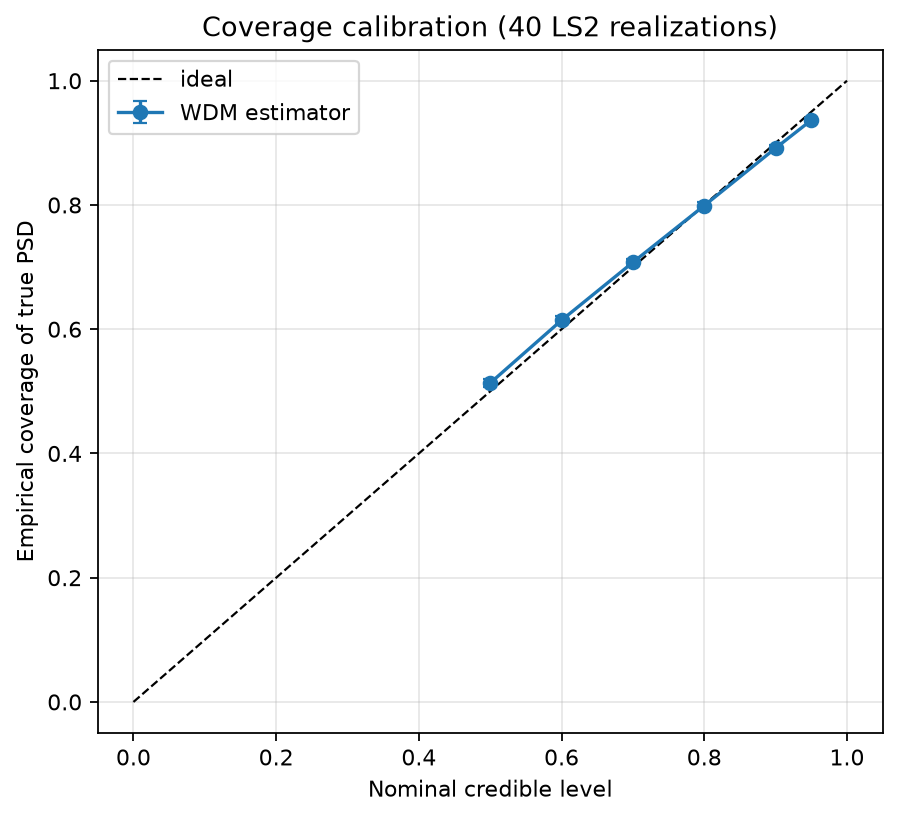
\includegraphics[width=0.55\linewidth]{figures/calibration.png}
    \caption{Coverage calibration over 40 LS2 realizations: empirical coverage of
    the true PSD versus the nominal credible level, against the ideal diagonal.}
    \label{fig:calibration}
\end{figure}

\begin{figure}
    \centering
    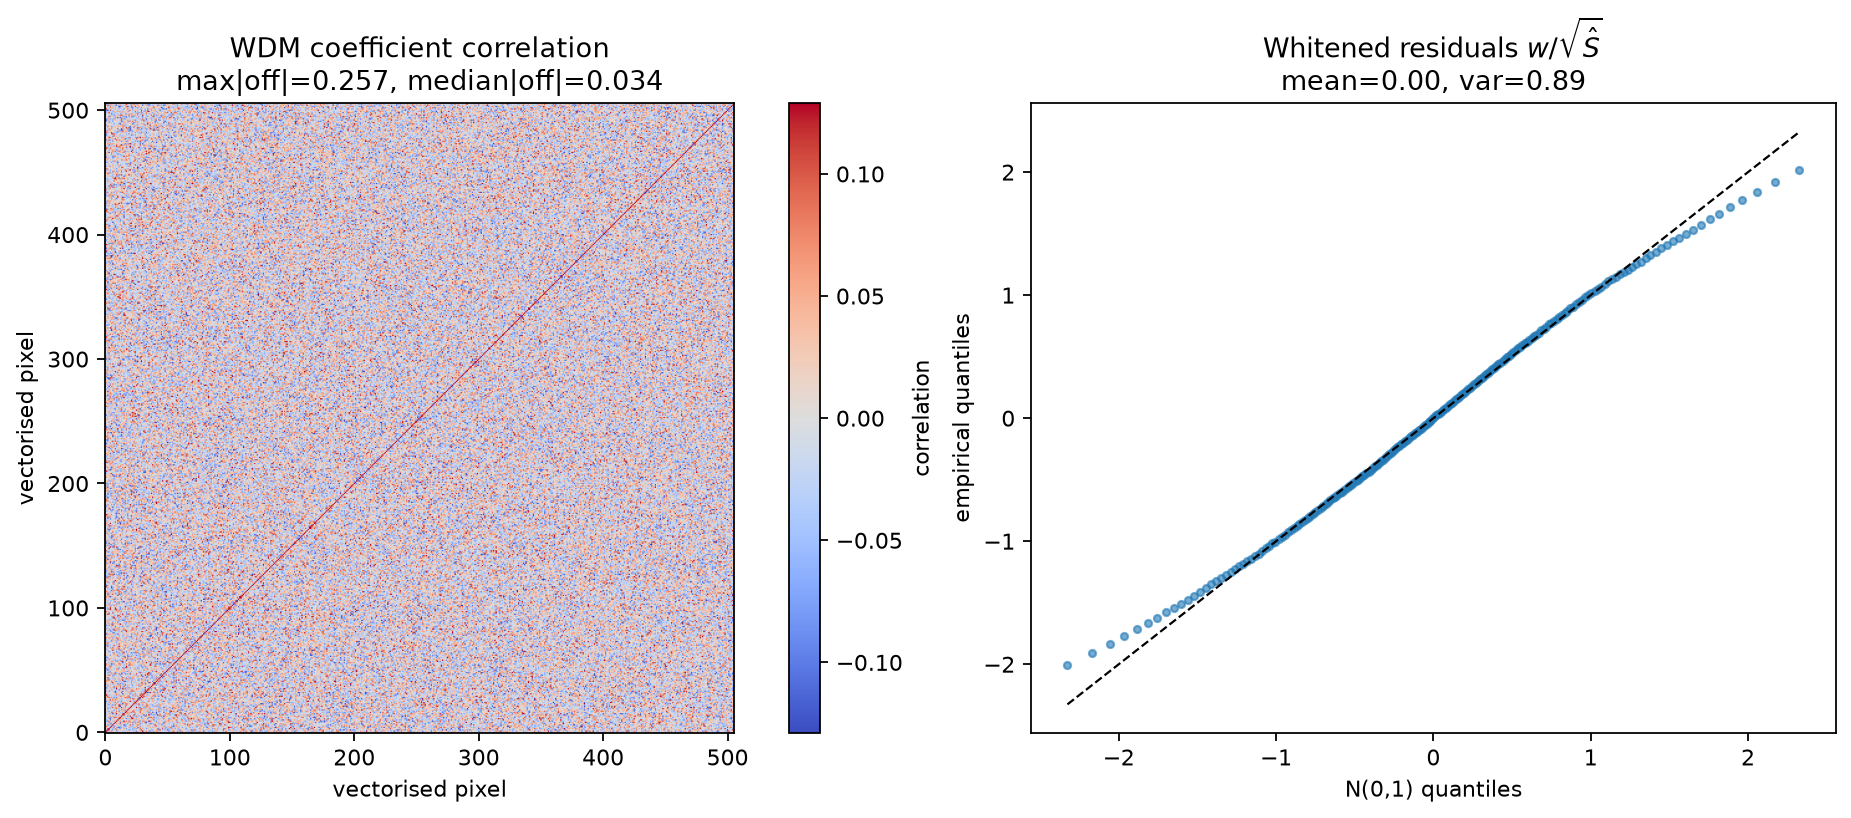
\includegraphics[width=0.95\linewidth]{figures/whittle_diagnostics.png}
    \caption{Left: empirical correlation of the vectorised trimmed WDM
    coefficients (white noise), quantifying the diagonal-Whittle approximation.
    Right: QQ plot of the whitened coefficients against a standard normal.}
    \label{fig:whittle_diag}
\end{figure}

For the non-stationary LISA budget, the simulated local power
(Fig.~\ref{fig:lisa_true}) shows the Galactic confusion foreground modulated in
time on top of the steeper instrument spectrum. The estimator recovers this
surface from a single noisy realization (Fig.~\ref{fig:lisa_surface}), and the
seasonal envelope is clearly tracked in a confusion-dominated channel
(Fig.~\ref{fig:lisa_channel}), where the posterior $90\%$ band contains the
analytic $S(u,f)$.

\paragraph{WDM versus the Tang dynamic Whittle.}
We compare against a faithful implementation of the Tang \emph{et al.} thinned
zigzag moving periodogram (Definitions~\ref{eq:MI}--\ref{eq:thinned_dynamic_whittle}):
the moving-periodogram ordinates are fit with the \emph{same} whitened P-spline
prior under the exponential dynamic-Whittle likelihood, so the comparison isolates
the time-frequency representation. Each estimate is rescaled to the analytic PSD
scale and scored on a common grid. On the smooth LS2 process the Tang dynamic
Whittle is the more accurate of the two (Fig.~\ref{fig:baseline}; median
$\mathrm{MSE}_{\log f}\approx 0.14$ versus $0.21$ for WDM at $n = 576$), and it
remains ahead across durations with the gap narrowing as the data grow
(Fig.~\ref{fig:duration}; both contract as power laws, with the ratio shrinking
from $\approx 1.6$ to $\approx 1.1$). Neither method produced a divergence.

The WDM estimator is therefore competitive but not superior for smooth locally
stationary spectra; its distinguishing advantages lie elsewhere. First, the
critically-sampled wavelet tiling is expected to help for sharply time-localized
or transient structure, which the moving periodogram smears across its window
(left to future work). Second, and most importantly, the WDM coefficient
likelihood retains phase and admits a signal mean, enabling the joint
signal-plus-noise global fit of Section~\ref{sec:joint} -- which a
power-periodogram dynamic Whittle, having discarded phase, cannot perform.

\subsection{Joint signal and noise inference}
\label{sec:joint}

Because the likelihood is Gaussian on the coefficients, it admits a coherent
signal mean, $w_{nm} \sim \mathcal{N}(h_{nm}(\bm\theta), S_{nm})$, so a signal and
the non-stationary noise PSD can be inferred jointly -- the wavelet-domain
analogue of a global fit. We demonstrate this with a galactic binary injected
into the modulated LISA noise of Section~\ref{sec:results}. In a single channel
the binary is a slowly chirping line $h(t) = a\,c(t) + b\,s(t)$ with cosine and
sine quadratures; since the WDM transform is linear, its coefficients are
$a\,g_{c,nm} + b\,g_{s,nm}$ for precomputed template coefficients, and we sample
the amplitudes $(a,b)$ jointly with the whitened P-spline noise prior. (The
quadrature amplitudes are well conditioned at a known frequency; a nonlinear
search over the binary frequency is multimodal and is deferred -- the
differentiable WDM backend and realistic TDI waveforms such as \texttt{jaxgb}
make it a natural extension.)

For a physically consistent demonstration we use realistic LISA data: the binary
TDI response is generated with \texttt{jaxGB} and the instrument noise PSD with
\texttt{lisatools}, in the \emph{same} TDI channel (X), generation (2), and units
(fractional frequency). This matching is essential -- scoring a generation-2
signal against generation-1.5 noise mis-estimates the SNR by a factor of a few --
and we verify it by recovering the same matched-filter SNR ($\approx 8$ for a
reference amplitude) from the time-domain data as from the frequency-domain
template, and by confirming the noise realisations reproduce the lisatools PSD.
We run a full observation \emph{year} ($1.83\times10^{5}$ samples on a
$366\times500$ WDM grid; the seasonal confusion modulation is a single physical
annual cycle). The non-stationary noise is the instrument floor plus the
modulated galactic confusion (also in TDI-X units), and a loud, resolvable binary
is injected at $1.5\,\mathrm{mHz}$ with SNR $\approx 80$ against the
confusion-dominated floor. The two \texttt{jaxGB} quadrature templates (initial
phases $0$ and $\pi/2$) span the monochromatic signal to machine precision, so the
linear amplitude model is exact and free of template mismatch. At this scale the
full posterior surface is not stored per sample; it is reconstructed from the
(small) eigen-coefficients in frequency chunks, so the estimator runs in bounded
memory and the fit completes in a few minutes.

The joint fit recovers the amplitude ($|A| = 0.999$ against an injected $1.0$)
with no divergences and cleanly separates the binary from the noise: the
recovered signal is a sharp line in the WDM plane and the residual is consistent
with noise (Fig.~\ref{fig:signal_decomp}). Crucially, ignoring the signal biases
the noise PSD -- a noise-only fit absorbs the binary power and overestimates the
local power in the signal channel, whereas the joint fit tracks the true annually
modulated noise PSD (Fig.~\ref{fig:signal_bias}). This is the core motivation for
joint estimation, and the reason the coefficient likelihood -- which retains
phase -- is preferable to a power periodogram. (The binary frequency is held at
its known value; a nonlinear frequency search is multimodal and is deferred.)

\begin{figure}
    \centering
    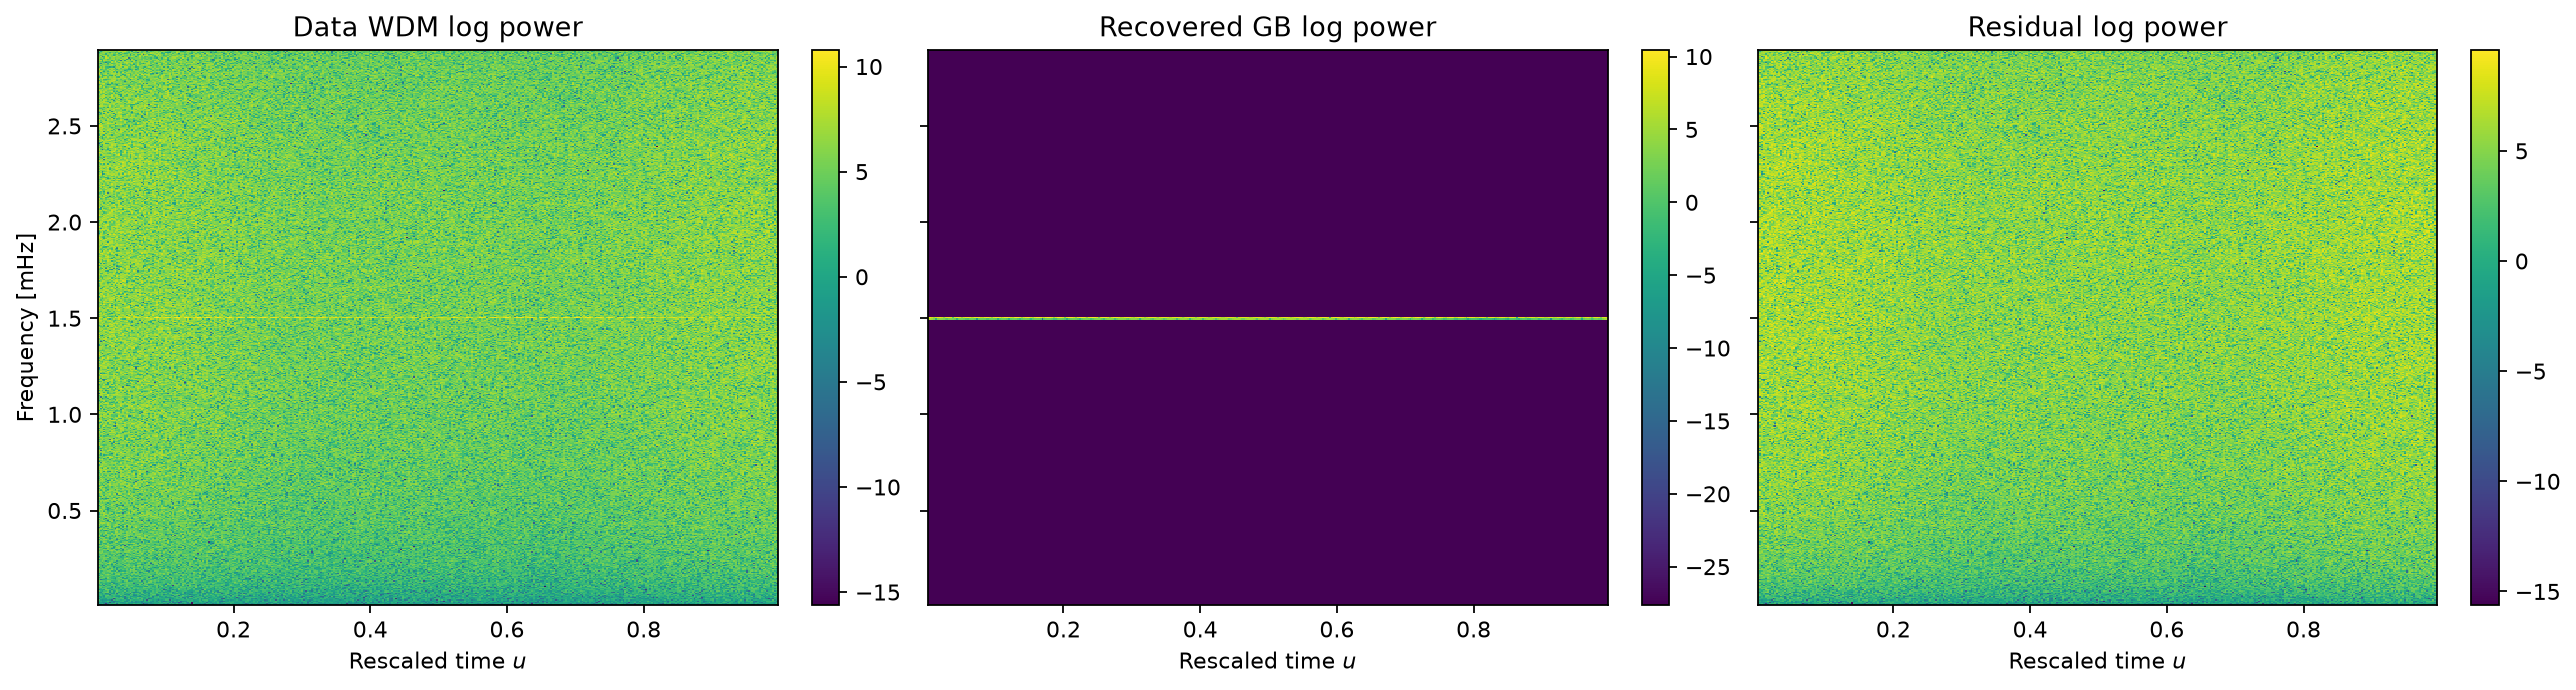
\includegraphics[width=0.98\linewidth]{figures/lisa_tdi_decomposition.png}
    \caption{Joint fit of a \texttt{jaxGB} galactic binary in modulated LISA TDI
    noise. Left: data WDM power, with the binary as a horizontal line. Centre: the
    recovered signal power. Right: the residual after subtracting the recovered
    signal, consistent with noise.}
    \label{fig:signal_decomp}
\end{figure}

\begin{figure}
    \centering
    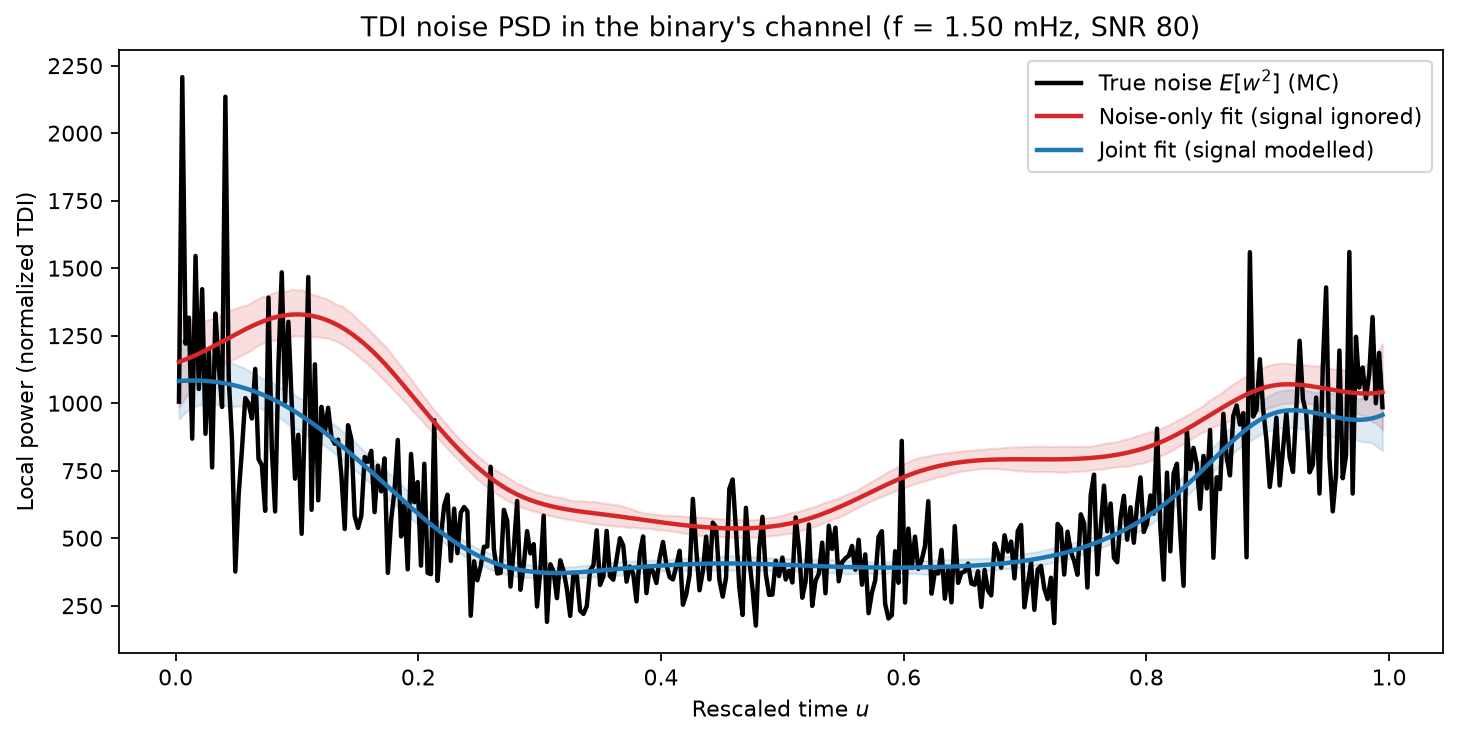
\includegraphics[width=0.75\linewidth]{figures/lisa_tdi_psd_bias.png}
    \caption{TDI noise PSD in the binary's channel. A noise-only fit (red) absorbs
    the signal power and is biased high; the joint fit (blue) recovers the true
    modulated noise PSD (black).}
    \label{fig:signal_bias}
\end{figure}

\begin{table}[ht]
\centering
\begin{tabular}{lccccc}
\hline
Study & repeats & $\mathrm{MSE}_{\log f}$ (vs $\mathbb{E}[w^2]$) & $\mathrm{MSE}_{\log f}$ (vs $C_m f_0$) & 90\% coverage & divergences \\
\hline
LS2  & 100 & $0.23\ [0.17, 0.31]$ & $0.30\ [0.21, 0.39]$ & $0.93$ & $0$ \\
LISA & 50  & $0.19\ [0.14, 0.26]$ & $0.18\ [0.13, 0.25]$ & $0.92$ & $0$ \\
\hline
\end{tabular}
\caption{Median $[p_5, p_{95}]$ log-PSD error, interval coverage, and total NUTS
divergences for the two simulation studies.}
\label{tab:results}
\end{table}

\begin{figure}
    \centering
    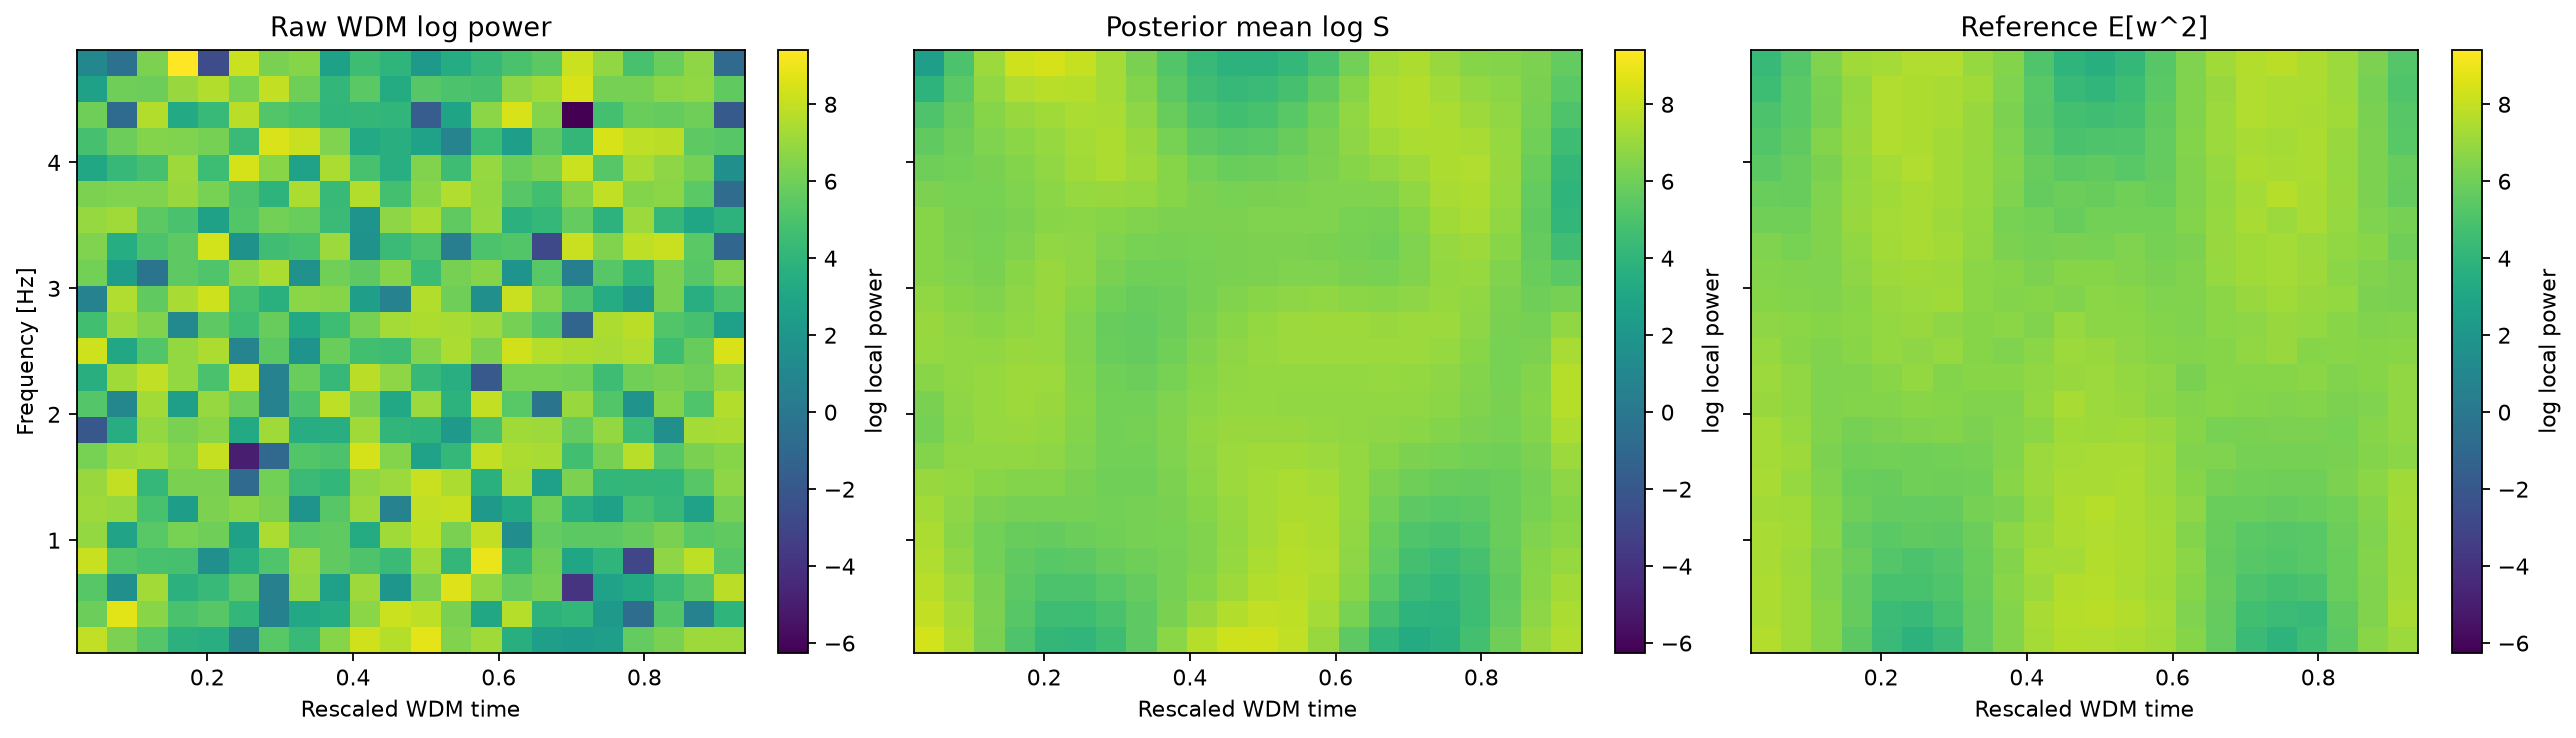
\includegraphics[width=0.9\linewidth]{figures/ls2_surface_example.png}
    \caption{Representative LS2 fit: raw WDM log power, posterior-mean
    $\log S(t,f)$, and the Monte Carlo $\mathbb{E}[w^2]$ reference.}
    \label{fig:ls2_surface}
\end{figure}

\begin{figure}
    \centering
    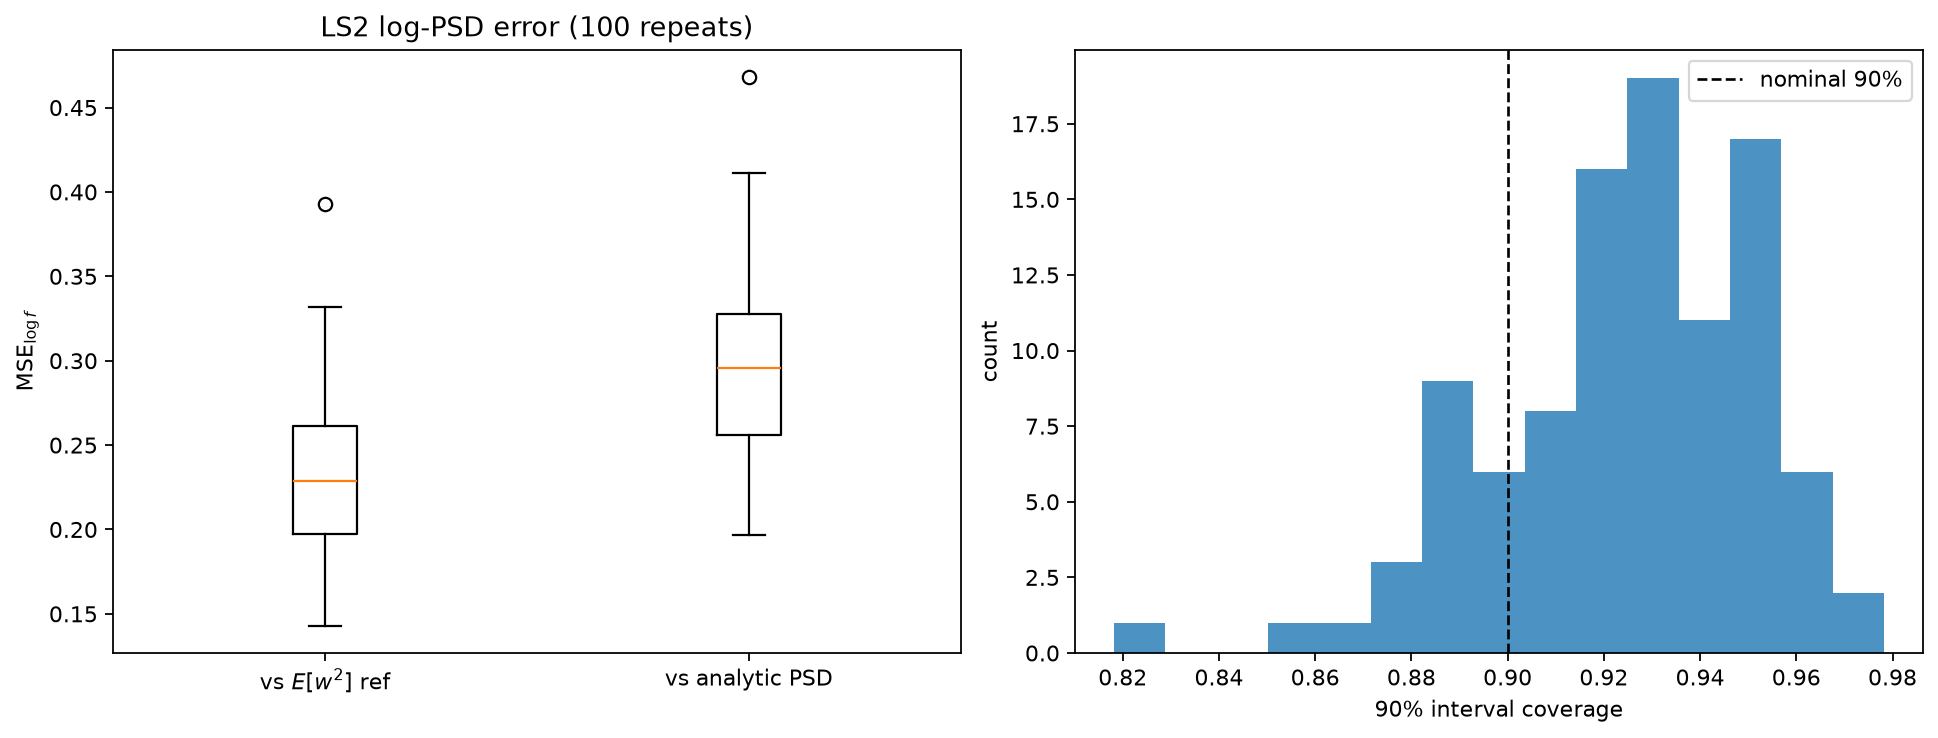
\includegraphics[width=0.9\linewidth]{figures/ls2_error_distribution.png}
    \caption{LS2 study over 100 realizations. Left: distribution of
    $\mathrm{MSE}_{\log f}$ against the Monte Carlo target and the calibrated
    analytic PSD. Right: posterior $90\%$ interval coverage (nominal dashed).}
    \label{fig:ls2_error}
\end{figure}

\begin{figure}
    \centering
    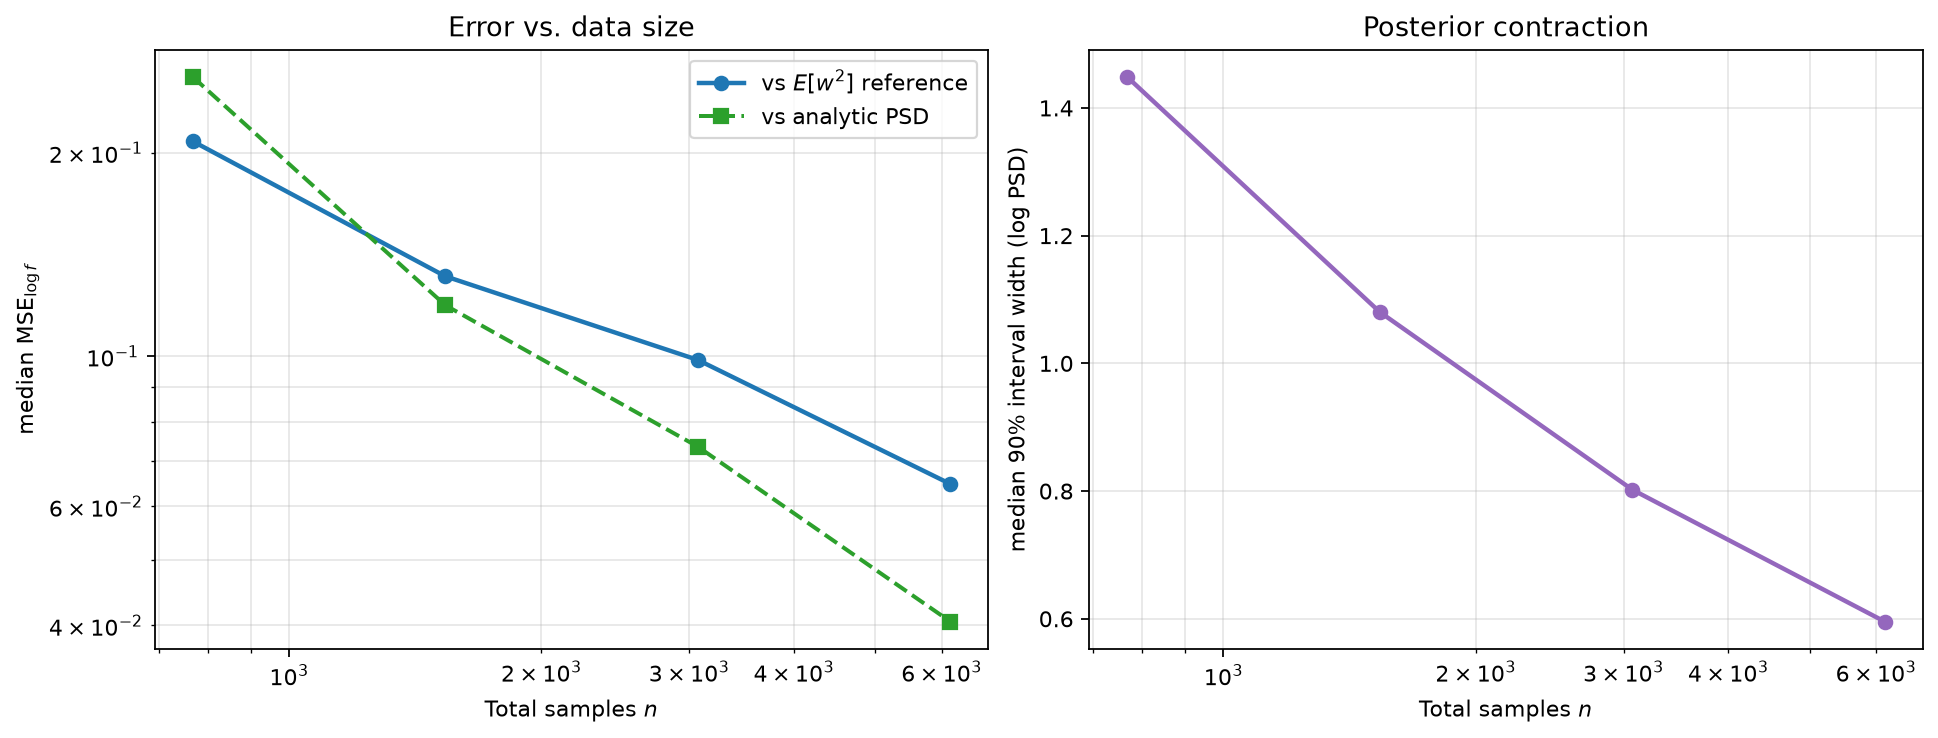
\includegraphics[width=0.9\linewidth]{figures/convergence.png}
    \caption{Posterior contraction for LS2 as the data grows (fixed model,
    increasing WDM time bins). Left: median $\mathrm{MSE}_{\log f}$ versus total
    samples $n$. Right: median posterior $90\%$ interval width versus $n$.}
    \label{fig:convergence}
\end{figure}

\begin{figure}
    \centering
    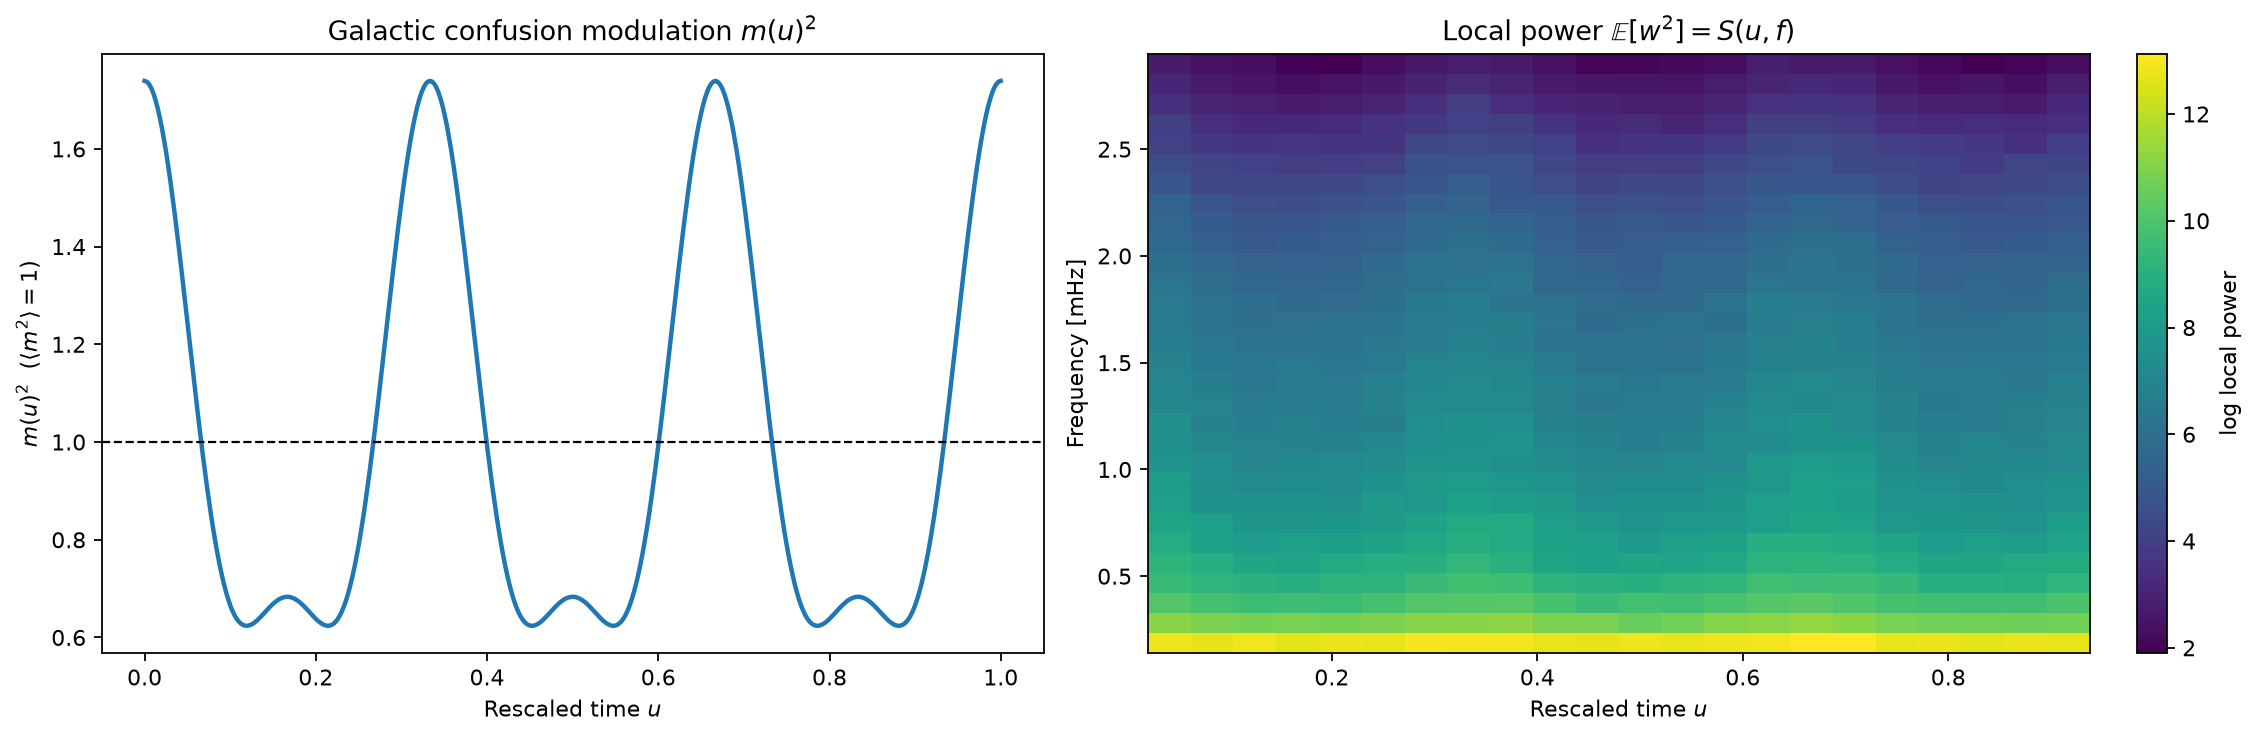
\includegraphics[width=0.9\linewidth]{figures/lisa_true_surface.png}
    \caption{Simulated non-stationary LISA noise: the seasonal modulation
    envelope $m(u)^2$ (left, normalized to $\langle m^2\rangle = 1$) and the
    resulting local power $S(u,f) = S_{\mathrm{inst}}(f) + m(u)^2
    S_{\mathrm{gal}}(f)$ (right).}
    \label{fig:lisa_true}
\end{figure}

\begin{figure}
    \centering
    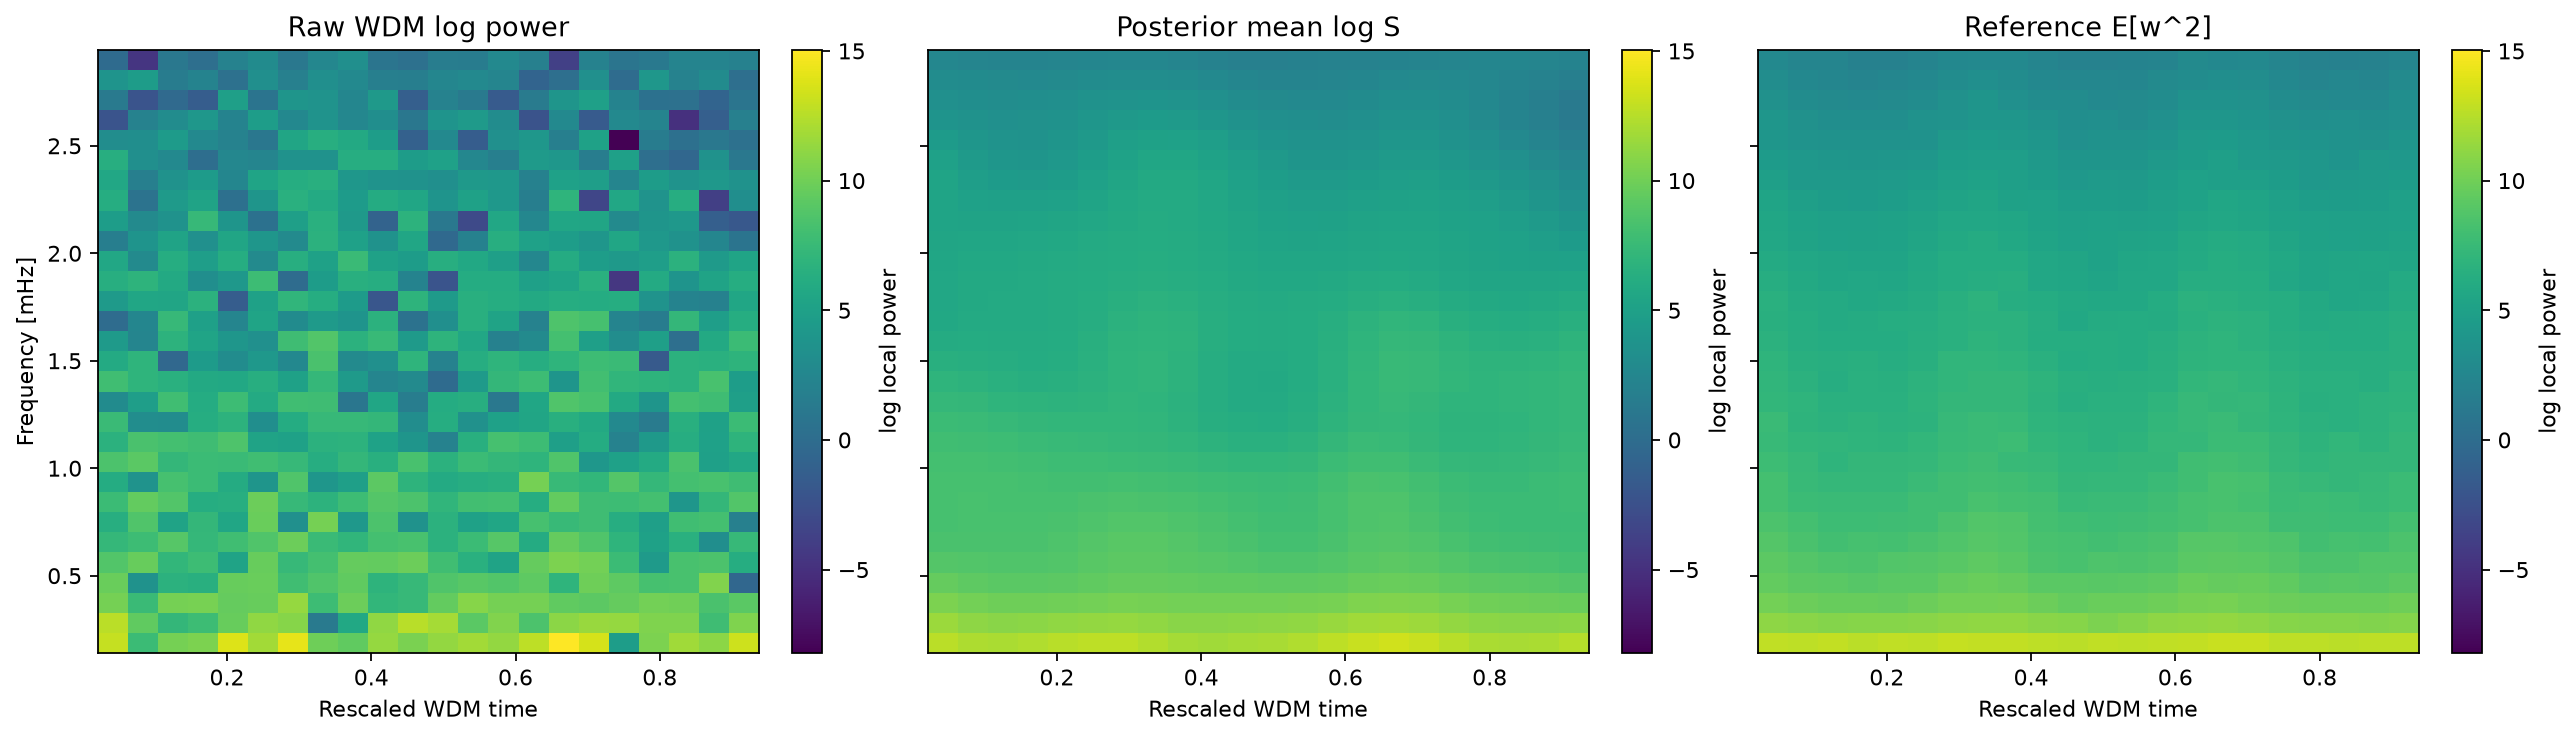
\includegraphics[width=0.9\linewidth]{figures/lisa_surface_comparison.png}
    \caption{Non-stationary LISA noise: raw WDM power, posterior-mean
    $\log S(u,f)$, and the Monte Carlo reference.}
    \label{fig:lisa_surface}
\end{figure}

\begin{figure}
    \centering
    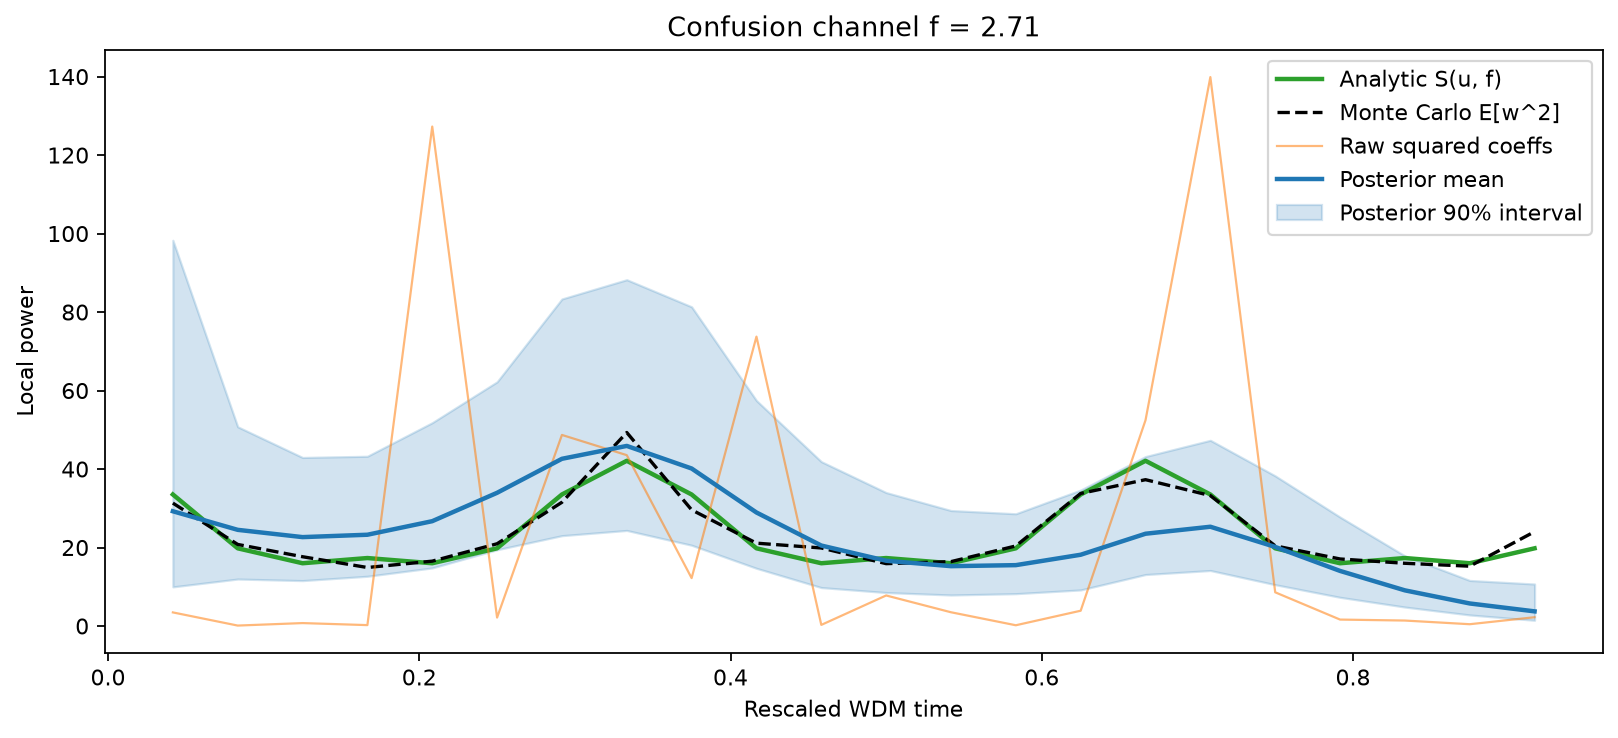
\includegraphics[width=0.6\linewidth]{figures/lisa_modulation_channel.png}
    \caption{Recovered seasonal modulation of the confusion foreground in a
    confusion-dominated channel, with the posterior $90\%$ interval.}
    \label{fig:lisa_channel}
\end{figure}

\begin{figure}
    \centering
    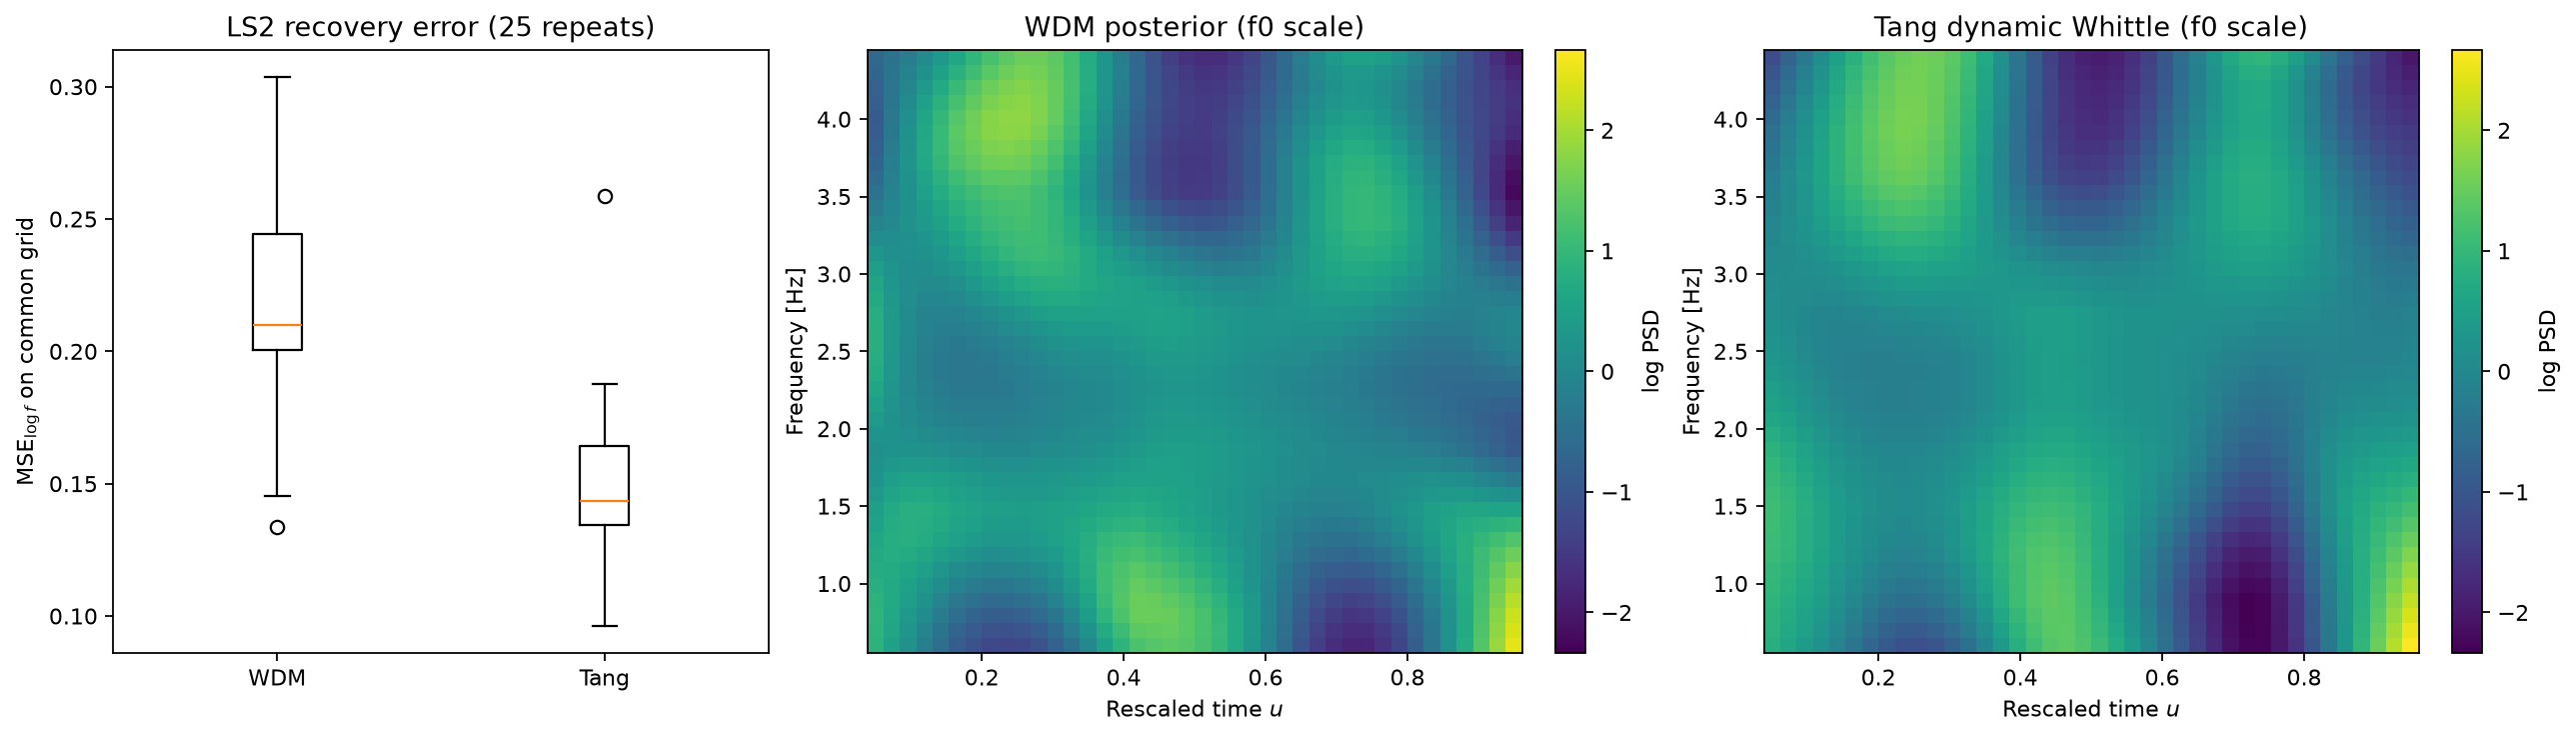
\includegraphics[width=0.95\linewidth]{figures/baseline_comparison.png}
    \caption{WDM estimator versus the Tang zigzag moving-periodogram dynamic
    Whittle on LS2, both using the same whitened P-spline prior. Left: distribution
    of $\mathrm{MSE}_{\log f}$ on a common grid over 25 realizations. Centre/right:
    representative posterior-mean surfaces (rescaled to the analytic PSD scale).}
    \label{fig:baseline}
\end{figure}

\begin{figure}
    \centering
    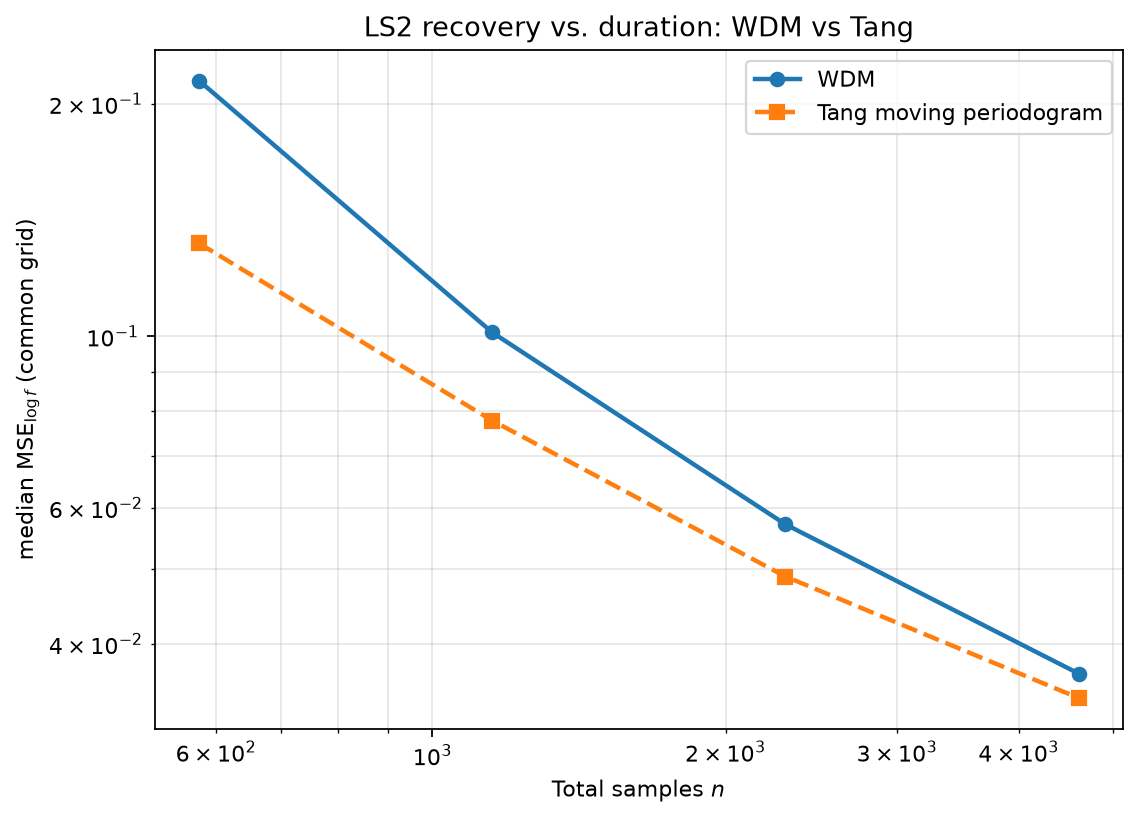
\includegraphics[width=0.7\linewidth]{figures/duration_comparison.png}
    \caption{LS2 recovery error versus total duration for the WDM estimator and
    the Tang dynamic Whittle. The Tang method is more accurate on this smooth
    process, with the gap narrowing as the data grow.}
    \label{fig:duration}
\end{figure}


\bibliographystyle{plainnat} 
\bibliography{refs}    


\end{document}
